\documentclass[a4paper]{article}
\usepackage[UTF8]{ctex}
\usepackage{geometry}
\usepackage{graphicx}
\usepackage{url}
\usepackage{multirow}
\usepackage{array}
\usepackage{booktabs}
\usepackage{url}
\usepackage{enumitem}
\usepackage{graphicx}
\usepackage{float}
\usepackage{amssymb}
\usepackage{amsmath}
\usepackage{subfig}
\usepackage{longtable}
\usepackage{pifont}
\usepackage{color}

\allowdisplaybreaks

\geometry{a4paper, scale=0.78}

% \begin{figure}[H]
%     \centering
%     \includegraphics[width=.55\textwidth]{E.png}
%     \caption{矩阵与列向量的乘法}
%     \label{fig:my_label_1}
% \end{figure}

% \left\{
% \begin{array}{ll}
%       x+2x+z=2 & \\
%       3x+8y+z=12 & \\
%       4y+z=2
% \end{array}
% \right.

% \begin{enumerate}[itemindent = 1em, itemsep = 0.4pt, parsep=0.5pt, topsep = 0.5pt]

% \end{enumerate}

%\stackrel{a}{\longrightarrow}

%\underbrace{}_{} %下括号

\title{Expectation Maximization 02 Derived Formula}
\author{Chen Gong}
\date{18 December 2019}

\begin{document}
\maketitle
机器学习中,所谓的模型实际上就可以看成是一堆的参数。根据极大似然估计的思想,我们要求解的对象的是:
\begin{equation}
    \theta_{MLE} = \log P(X|\theta)
\end{equation}

其中,$X$为observed data;$Z$为latent data;$(X,Z)$为complete data;$\theta$为parameter。

那么,EM公式就被我们描述为:
\begin{equation}
\theta^{(t+1)} = \arg\max_{\theta} \int_Z \log P(X,Z|\theta)P(Z|X,\theta^{(t)}) dZ    
\end{equation}

EM算法可以被我们分解成E-step和M-step两个部分。

E-step:
\begin{equation}
    P(Z|X,\theta^{(t)}) \longrightarrow \mathbb{E}_{Z\sim P(Z|X,\theta^{(t)})}\left[ \log P(X,Z|\theta) \right]
\end{equation}

M-step:
\begin{equation}
    \theta^{(t+1)} = \arg\max_{\theta} \mathbb{E}_{Z\sim P(Z|X,\theta^{(t)})}\left[ \log P(X,Z|\theta) \right]
\end{equation}

前面我们已经证明了EM算法的收敛性了,也就是:
\begin{equation}
    \log P(X|\theta^{(t+1)}) \geq \log P(X|\theta^{(t)})
\end{equation}

收敛性告诉了我们算法确实是有效的,我们可以放心的去使用它。而大家会不会觉得这个公式的得来有点懵逼?懵逼就对了,那么下一步,我们的目标就是要推导出EM算法究竟是怎么来的,给出一个理论的证明。

\section{从KL Divergence进行分析}
这是个什么东西呢?中文名字叫做“证据下界”。这个名字读起来似乎有一点点奇怪。我们首先看看它是怎么来的。首先,我们定义一个有关于表示层$Z$的表示层变量$q(Z)$,$q(Z)$可以表示任何一个变量。
\begin{equation}
    \begin{split}
        \log P(X|\theta) 
        = & \log P(X,Z|\theta) - \log P(Z|X,\theta) \\
        = & \log \frac{P(X,Z|\theta)}{Q(Z)} - \log \frac{P(Z|X,\theta)}{Q(Z)} \\
    \end{split}
\end{equation}

两边同时对于$Q(Z)$求期望,我们可以得到:

左边:
\begin{equation}
    \begin{split}
    \int_Z Q(Z)\log P(X|\theta)  dZ 
    = &  \log P(X|\theta) \int_Z Q(Z) dZ \\    
    = &  \log P(X|\theta) \cdot 1 \\
    = &  \log P(X|\theta)
    \end{split}
\end{equation}

右边:
\begin{equation}
    \begin{split}
        \underbrace{\int_Z Q(Z) \log \frac{P(X,Z|\theta)}{Q(Z)}dZ}_{ELBO} - 
        \underbrace{\int_Z Q(Z) \log \frac{P(Z|X,\theta)}{Q(Z)}dZ}_{KL}
    \end{split}
\end{equation}

所以,实际上,$\log P(X|\theta) = ELBO + KL(Q||P)$。其中,$P(Z|X,\theta)$为后验分布(Posterior)。并且,KL散度的值一定是大于零的。所以,$\log P(X|\theta) \geq ELBO$,当且仅当$P(Z|X,\theta) = Q(Z)$时等号成立。

{\color{red} EM算法的一个想法就是想让ELBO不断的增加,从而使$\log P(X|\theta)$不断的变大的一种攀爬的迭代方法。}

那么,我们对下界进行优化,使下界尽可能的变大,就可以使目标函数不断的上升,那么我们可以得到:
\begin{equation}
    \hat{\theta} = \arg\max_{\theta} ELBO = \arg\min_{\theta} -\int Q(Z)\log \frac{P(X,Z|\theta)}{Q(Z)}dZ
\end{equation}

而这里的$Q(Z)$的分布我们怎么得到呢?这里我们就要来讲一讲EM算法的一个核心的理解了。首先我们给出这个理解的图示结果,再对这个图来进行讲解:
\begin{figure}[H]
    \centering
    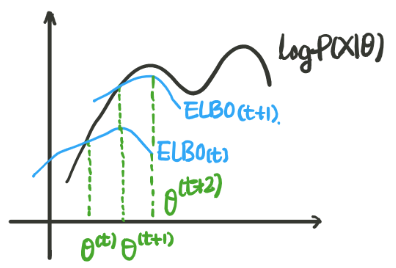
\includegraphics[width=.40\textwidth]{微信图片_20191218203645.png}
    \caption{EM算法迭代流程图}
    \label{fig:my_label_1}
\end{figure}

由于我们的目标是最大化ELBO。这个下界我们怎么优化?因为我们需要优化的是ELBO的参数$\theta$。那么,对于某一个时刻的$\theta^{(t)}$,我们可以的得到一个关于$\theta$的函数:
\begin{equation}
    \log P(X|\theta^{(t)}) = \int_Z Q(Z) \log \frac{P(X,Z|\theta)}{Q(Z)}dZ - \int_Z Q(Z) \log \frac{P(Z|X,\theta^{(t)})}{Q(Z)}dZ
\end{equation}

由于想让$\int_Z Q(Z) \log \frac{P(X,Z|\theta)}{Q(Z)}dZ$更大。由于$\log P(X|\theta^{(t)})$是一个定值,那么也就是想让KL散度的值越小。所以,我们想让KL散度的值为零,也就是让$Q(Z) = P(X,Z|\theta^{(t)})$。这样我们在固定了$\theta^{(t)}$之后就得到了一个ELBO关于$\theta$的函数。然后我们找到这个函数令值最大的$\theta^{(t+1)}$后开始进行下一步迭代。实际上我们的目的就是在不断的优化ELBO,使ELBO不断的变大,那么我们想要的结果自然也就变大了,这是一个间接优化的方法。所以,我们紧接着公式(9)进行推导:
\begin{equation}
    \begin{split}
        \hat{\theta} 
        = & \arg\max_{\theta} \int Q(Z)\log \frac{P(X,Z|\theta)}{Q(Z)}dZ \\ 
        = & \arg\max_{\theta} \int P(X,Z|\theta^{(t)})\log \frac{P(X,Z|\theta)}{P(X,Z|\theta^{(t)})}dZ \\
        = & \arg\max_{\theta} \int P(X,Z|\theta^{(t)})\log P(X,Z|\theta) - P(X,Z|\theta^{(t)})P(X,Z|\theta^{(t)})dZ \\
    \end{split}
\end{equation}

由于,$P(X,Z|\theta^{(t)})P(X,Z|\theta^{(t)})$与$\theta$的求解无关。所以我们可以直接省略掉。那么下一步的$\theta^{(t+1)}$的表达自然也就是:
\begin{equation}
    \begin{split}
        \theta^{(t+1)} 
        = & \arg\max_{\theta} \int_Z P(X,Z|\theta^{(t)})\log P(X,Z|\theta)dZ \\
        = & \arg\max_{\theta} \mathbb{E}_{Z\sim P(Z|X,\theta^{(t)})}\left[ \log P(X,Z|\theta) \right]
    \end{split}
\end{equation}

而这个公式(12),实际上就是我们之前直接给出的公式(3)和公式(4)。

\section{从Jensen Inequality的角度进行分析}
首先,我们介绍一下什么是Jensen Inequality。实际上,进行过一些机器学习理论研究的同学,都应该听说过这个概念。在这里我们做一个简述。首先我们需要保证函数是一个凸函数,下面我们来画一个凸函数:
\begin{figure}[H]
    \centering
    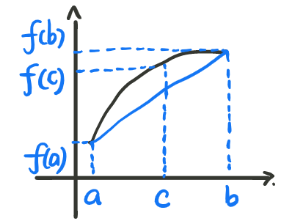
\includegraphics[width=.40\textwidth]{微信图片_20191218214143.png}
    \caption{凸函数示意图}
    \label{fig:my_label_1}
\end{figure}

那么对于一个$t\in [0,1]$,$c = ta+(1-t)b$,我们都可以得到:
\begin{equation}
    f(c) = f[ta+(1-t)b] \geq tf(a)+(1-t)f(b)
\end{equation}

当$t = \frac{1}{2}$时,我们可以得到:
\begin{equation}
    f(\frac{(a+b)}{2}) \geq \frac{1}{2}[f(a)+f(b)] \qquad f[E] \geq E[f]
\end{equation}

所以,我们可以利用Jensen Inequality进行推导:
\begin{equation}
    \begin{split}
        \log P(X|\theta) 
        = & \log \int_z P(X,Z|\theta) dZ \\
        = & \log \int_z Q(Z) \frac{P(X,Z|\theta)}{Q(Z)} dZ \\
        = & \log \mathbb{E}_{Z\sim Q(Z)}\left[ \frac{P(X,Z|\theta)}{Q(Z)} \right]\\
        \geq & \mathbb{E}_{Z\sim Q(Z)}\left[ \log \frac{P(X,Z|\theta)}{Q(Z)} \right] \\
    \end{split}
\end{equation}

根据Jensen Inequality的定义,当$\frac{P(X,Z|\theta)}{Q(Z)} = C$时可以取得等号。不知道,大家有没有发现这里的$\mathbb{E}_{Z\sim Q(Z)}\left[ \log \frac{P(X,Z|\theta)}{Q(Z)} \right]$实际上就是$\int_Z Q(Z) \log \frac{P(X,Z|\theta)}{Q(Z)}dZ$,也就是之前在KL Divergence角度进行分析时得到的ELBO。

毫无疑问,当我们取等时,可以达到最大。所以有,
\begin{gather}
    \frac{P(X,Z|\theta)}{Q(Z)} = C \\
    Q(Z) = \frac{1}{C} P(X,Z|\theta) \\
    \int_Z Q(Z) dZ = \frac{1}{C} \int_Z P(X,Z|\theta) dZ \\
    1 = \frac{1}{C} P(X|\theta)
\end{gather}

所以,我们就可以得到:
\begin{equation}
    Q(Z) = \frac{P(X,Z|\theta)}{P(X|\theta)} = P(Z|X,\theta)
\end{equation}

所以,大家有没有惊奇的发现,这个$Q(Z)$实际上就是Posterior。当时我们随便引入的一个分布$Q(Z)$,没想到当它取等的时候就是后验分布。那么像不断去优化这个ELBO,从而使得$\log P(X|\theta)$的值不断的增加。由于,我们是迭代式的上升,这里的$Q(Z) = P(Z|X,\theta^{(t)})$,而$\theta^{(t)}$是上一次迭代得到的,我们可以认为是一个常数。所以,
\begin{equation}
    \mathbb{E}_{Z\sim Q(Z)}\left[ \log \frac{P(X,Z|\theta)}{Q(Z)} \right] = \mathbb{E}_{Z\sim Q(Z)}\left[ \log \frac{P(X,Z|\theta)}{P(Z|X,\theta^{(t)})} \right]
\end{equation}

所以,
\begin{equation}
    \theta^{(t+1)} = \arg\max_{\theta} \mathbb{E}_{Z\sim Q(Z)}\left[ \log \frac{P(X,Z|\theta)}{P(Z|X,\theta^{(t)})} \right]
\end{equation}

所以,从Jensen Inequality的角度,我们仍然可以得到EM算法的核心表达式。

\section{小结}
在最后,我们再来来梳理一下EM算法的实现思想。我们的目标是想使$P(X|\theta)$似然函数值最大。但是,很不幸,我们直接优化非常的难。所以,我们想到了一个优化下降的方法。对于,每一个$\theta^{(t)}$时,我们可以计算得到下界为:$\mathbb{E}_{Z\sim Q(Z)}\left[ \log \frac{P(X,Z|\theta)}{P(Z|X,\theta^{(t)})} \right]$,令这个值最大我们就得到了,想要求得的$\theta^{(t+1)}$。然后,按这个思路,不断的进行迭代。

\end{document}
